\pdfminorversion=7
\documentclass[a4paper,final]{article}
\usepackage[14pt]{extsizes}
\usepackage[T2A]{fontenc}
\usepackage[utf8]{inputenc}
\usepackage[russian]{babel}

\addto\captionsrussian{\renewcommand{\figurename}{Рис.}}

% --- Math ---
\usepackage{amsmath,amssymb,amsfonts}
\usepackage{nccmath}

% --- Page geometry ---
\usepackage[left=20mm, top=20mm, right=20mm, bottom=20mm, footskip=10mm]{geometry}

% --- Text/layout helpers ---
\usepackage{ragged2e}
\usepackage{setspace}
\usepackage{indentfirst}

% --- Graphics ---
\usepackage{graphicx}
\DeclareGraphicsExtensions{.jpg,.png,.pdf}
\usepackage{float}
\usepackage{wrapfig}
\usepackage{tikz}
\usepackage{pgfplots}
\pgfplotsset{compat=1.18}

% --- Captions ---
\usepackage[font=small,singlelinecheck=false,justification=centering,labelsep=period]{caption}

% --- Lists ---
\usepackage{enumitem}

% --- Hyperlinks ---
\usepackage{hyperref}
\hypersetup{colorlinks=true, linkcolor=blue, urlcolor=blue}

% --- Code listings ---
\usepackage{xcolor}
\usepackage{listings}

\definecolor{codegreen}{rgb}{0,0.6,0}
\definecolor{codegray}{rgb}{0.5,0.5,0.5}
\definecolor{codepurple}{rgb}{0.58,0,0.82}
\definecolor{backcolour}{rgb}{0.95,0.95,0.92}

% --- CLIPS language definition for listings ---
\lstdefinelanguage{CLIPS}{
	keywords={deffunction, defrule, assert, retract, printout,
	          read, bind, while, do, halt, declare, not, or, and,
	          if, then, else, member\$, lowcase, lexemep, eq, salience},
	morestring=[b]",
	morecomment=[l]{;},
	sensitive=false
}

\lstdefinestyle{mystyle}{
	backgroundcolor=\color{backcolour},
	commentstyle=\color{codegreen},
	keywordstyle=\color{magenta},
	numberstyle=\tiny\color{codegray},
	stringstyle=\color{codepurple},
	basicstyle=\ttfamily\footnotesize,
	breaklines=true,
	breakatwhitespace=false,
	captionpos=b,
	keepspaces=true,
	numbers=left,
	numbersep=5pt,
	showspaces=false,
	showstringspaces=false,
	showtabs=false,
	tabsize=4,
	columns=fullflexible,
	extendedchars=true,
	inputencoding=utf8,
	literate=
	{•}{{-}}1
	{–}{{-}}1
	{—}{{-}}1
}

\lstset{style=mystyle}
\renewcommand{\lstlistingname}{Листинг}
\DeclareUnicodeCharacter{202F}{\,}
\sloppy

% --- Other document tweaks ---
\renewcommand{\arraystretch}{1.4}
\parindent=24pt
\parskip=0pt
\tolerance=2000
\flushbottom

\addto\captionsrussian{\def\refname{Список использованной литературы}}

\begin{document}
	\begin{center}
		\normalsize\bf{{МИНИСТЕРСТВО НАУКИ И ВЫСШЕГО ОБРАЗОВАНИЯ РОССИЙСКОЙ ФЕДЕРАЦИИ}

			\hfill \break
			федеральное государственное автономное образовательное учреждение высшего образования\\ «Санкт-Петербургский политехнический университет\\ Петра Великого»\\[10pt]}
		\hfill \break
		\normalsize{Институт компьютерных наук и кибербезопасности}\\[10pt]

		\normalsize{Высшая школа технологий и искусственного интеллекта}\\[10pt]

		\normalsize{Направление: 02.03.01 Математика и компьютерные науки}\\
		\vspace{50pt}

		\vspace{1pt}
		\begin{center}
Отчет по курсовой работе\\
по дисциплине «Теория графов»\\
Реализация экспертной системы:\\
«Выбор животного на основе заданных характеристик»

		\end{center}

		\hfill \break
		\hfill \break
	\end{center}
	\small{ \bf
		\begin{tabular}{lrrl}
			\!\!\!Студент, & \hspace{0cm} & & \\
			\!\!\!группа 5130201/40001 & \hspace{1.5cm} & \underline{\hspace{3cm}} & \hspace{-0.3cm}Ови Мд Шамин Ясир  \\\\
			\!\!\!Преподаватель, & \hspace{1cm} & \\
			\!\!\! & \hspace{0.1cm} & \underline{\hspace{3cm}} &  Востров Алексей Владимирович\\\\
			&&\hspace{3.5cm}
		\end{tabular}
		\begin{flushright}
			<<\underline{\hspace{1cm}}>>\underline{\hspace{2.5cm}} 2026г.
		\end{flushright}
	}

	\hfill \break
	\hfill \break
	\begin{center} \small\bf{Санкт-Петербург, 2026} \end{center}
	\thispagestyle{empty}
	% END OF TITLE PAGE

\newpage
\renewcommand{\contentsname}{Содержание}
\tableofcontents


\newpage
\section*{Введение}
\addcontentsline{toc}{section}{Введение}

Экспертные системы~--- системы, основанные на моделях знаний из определённых предметных областей.

Экспертная система заключает в себе знания высококвалифицированного специалиста в определённой предметной области и используется для консультаций, помощи в принятии сложных решений, для решения неформализованных задач.

В данной работе необходимо реализовать экспертную систему в среде CLIPS на основе продукционной модели в области «Выбор домашнего животного на основе заданных характеристик».

Минимальный размер бинарного дерева: 4~яруса, 30~узлов.


\newpage
\section{Предметная область}

В качестве предметной области был выбран «выбор домашнего животного на основе заданных характеристик». Данная область знаний включает в себя информацию, которая используется для подбора подходящего питомца в зависимости от образа жизни, жилищных условий и личных предпочтений владельца.

Факты, используемые для классификации, выбраны таким образом, чтобы позволить пользователю однозначно определить наиболее подходящего питомца. Ключевые характеристики для классификации: важность ежедневного общения, готовность к прогулкам и дрессировке, предпочтение активного или пассивного питомца, допустимость ночной активности, желание аквариума или птицы.

\subsection*{Почему была выбрана данная тема}

Выбор домашнего животного является типичной неформализованной задачей: не существует единого алгоритма решения, результат зависит от многих субъективных факторов~--- образа жизни, жилищных условий, наличия времени и личных предпочтений. Такие задачи идеально подходят для продукционной модели экспертной системы, поскольку каждый характерный признак можно однозначно выразить в виде правила ЕСЛИ-ТО:

\begin{quote}
ЕСЛИ (важно ежедневное общение) И (есть время на прогулки)\\
И (подходит крупное животное)\\
ТО рекомендуется Собака
\end{quote}

Тема актуальна: в Бангладеш за последние три года количество владельцев домашних животных более чем удвоилось. Объём рынка зоотоваров составляет около~2~млрд така в год с ежегодным ростом свыше~20\%~\cite{dailystar}.

\subsection*{Как были выбраны животные}

Все 16~животных, включённых в систему, выбраны на основании их популярности и доступности в Бангладеш, что подтверждается достоверными источниками:

\begin{itemize}
	\item По данным The Daily Star (Бангладеш)~\cite{dailystar}, около~90\% владельцев питомцев держат кошек~--- это самый популярный питомец в стране. Рынок зоотоваров растёт более чем на~20\% в год.

	\item Согласно академическому исследованию 2024~года (ResearchGate)~\cite{researchgate1}: кошки~--- 56{,}2\% владельцев, птицы~--- 35{,}5\%, собаки~--- 11{,}1\%, кролики~--- 5\% от всех питомцев.

	\item По данным торговой площадки Bikroy.com~\cite{bikroy} (крупнейший онлайн-рынок Бангладеш), в активной продаже представлены: собаки, кошки, кролики, попугаи, голуби, майны, канарейки, аквариумные рыбки, черепахи, хомяки, морские свинки, декоративные крысы, кореллы, волнистые попугайчики, неразлучники, золотые рыбки.

	\item По данным BdFISH~\cite{bdfish}, в Бангладеш насчитывается более~70 видов декоративных и аквариумных рыб, активно продающихся в зоомагазинах Дакки и Раджшахи.

	\item Зоорынок Катабон (Dhaka)~\cite{katabon} подтверждает доступность всех~16 видов животных в физических магазинах.
\end{itemize}

Таким образом, критерий отбора: широко распространённые, доступные и безопасные домашние животные в Бангладеш, пригодные для содержания в квартире или частном доме.

\subsection*{Список животных (факты экспертной системы)}

Данный перечень представляет собой список всех возможных результатов работы экспертной системы:

\begin{enumerate}
	\item Собака
	\item Кролик
	\item Кошка
	\item Морская свинка
	\item Хомяк
	\item Декоративная крыса
	\item Голубь
	\item Майна
	\item Аквариумные рыбки
	\item Золотая рыбка
	\item Черепаха
	\item Корелла
	\item Попугай
	\item Канарейка
	\item Неразлучник
	\item Волнистый попугайчик
\end{enumerate}


\newpage
\section{Математическое описание}

\subsection{Экспертная система и её особенности}

\textbf{Экспертная система}~--- это компьютерная система, которая использует знания экспертов в определённой области для решения сложных проблем и предоставления рекомендаций или прогнозов.

Экспертные системы главным образом основаны на эвристическом поиске решения, а не на исполнении известного алгоритма. В этом одно из главных преимуществ технологии экспертных систем перед традиционным подходом к разработке программ. Именно это и позволяет им так хорошо справляться с поставленными перед ними задачами.

Экспертная система работает в двух основных режимах:
\begin{itemize}
	\item в режиме приобретения знаний;
	\item в режиме решения задачи (называемом также режимом консультаций, или режимом использования экспертной системы).
\end{itemize}

\textbf{В режиме приобретения знаний} работу с экспертной системой осуществляет эксперт при посредничестве инженера по знаниям. В этом режиме эксперт, используя компонент приобретения знаний, наполняет систему знаниями (данными), которые, в свою очередь, позволяют системе в режиме решения уже без участия эксперта решать задачи из данной предметной области.

\textbf{В режиме решения задачи} (или так называемом режиме консультации) общение с экспертными системами осуществляет непосредственно конечный пользователь, которого интересует конечный итог работы и иногда способ его получения. В зависимости от назначения экспертной системы пользователь не обязательно должен быть специалистом в данной проблемной области. В этом случае он обращается к экспертным системам за результатом, не имея достаточных знаний для получения результатов.

Компоненты структуры экспертной системы:

\begin{itemize}
	\item \textbf{Интерфейс пользователя}: обеспечивает взаимодействие между пользователем и экспертной системой. Он может быть графическим, текстовым или голосовым, позволяя пользователю задавать вопросы, получать ответы, вводить данные и взаимодействовать с системой. Интерфейс должен быть интуитивно понятным и удобным для пользователей.

	\item \textbf{База знаний}: знания~--- это правила, законы, закономерности, полученные в результате профессиональной деятельности в пределах предметной области. База знаний~--- база данных, содержащая правила вывода и информацию о человеческом опыте и знаниях в некоторой предметной области. Другими словами, это набор таких закономерностей, которые устанавливают связи между вводимой и выводимой информацией.

	\item \textbf{Данные}: данные~--- это совокупность фактов и идей, представленных в формализованном виде. На данных основываются закономерности для предсказания, прогнозирования. Продвинутые интеллектуальные системы способны учиться на основе этих данных, добавляя новые знания в базу знаний.

	\item \textbf{Механизм логического вывода данных (Подсистема вывода)}: выполняет анализ и получение новых знаний исходя из сопоставления исходных данных из базы данных и правил из базы знаний. Механизм логического вывода концептуально можно представить в виде $\langle A,\,B,\,C,\,D \rangle$:
	\begin{itemize}
		\item $A$~--- функция выбора из базы знаний и из базы данных закономерностей и фактов соответственно;
		\item $B$~--- функция проверки правил, результатом которой определяется множество фактов из базы данных, к которым применимы правила;
		\item $C$~--- функция, которая определяет порядок применения правил, если в результате правила указаны одинаковые факты;
		\item $D$~--- функция, которая применяет действие.
	\end{itemize}

	\item \textbf{Машина логического вывода}: является программным компонентом, который определяет антецеденты правил (если таковые имеются), которые выполняются согласно фактам. Для этого машина логического вывода выполняет следующие действия:
	\begin{itemize}
		\item выбирает правила, которым соответствуют факты;
		\item распределяет выбранные правила по приоритетам;
		\item выполняет правило с высшим приоритетом.
	\end{itemize}

	\item \textbf{Интеллектуальный редактор}: обеспечивает режим пополнения базы знаний. Позволяет эксперту при посредничестве инженера по знаниям вводить новые правила и факты в систему.
\end{itemize}


\subsection{Продукционная модель представления знаний}

По своей сути продукционные модели знаний близки к логическим моделям, что позволяет организовать весьма эффективные процедуры логического вывода данных.

Традиционная продукционная модель знаний включает в себя следующие базовые компоненты:

\begin{enumerate}
	\item набор правил (или продукций), представляющих базу знаний продукционной системы;
	\item рабочую память, в которой хранятся исходные факты, а также факты, выведенные из исходных фактов при помощи механизма логического вывода;
	\item сам механизм логического вывода, позволяющий из имеющихся фактов, согласно имеющимся правилам вывода, выводить новые факты.
\end{enumerate}

\begin{itemize}
	\item В основе продукционной модели представления знаний находится конструктивная часть~--- продукция~(правило):\\[4pt]
	IF $\langle$\textit{условие}$\rangle$,\; THEN $\langle$\textit{действие №1}$\rangle$,\; ELSE $\langle$\textit{действие №2}$\rangle$

	\item Продукция состоит из двух частей: условие~--- антецедент, действие~--- консеквент.

	\item Условия можно сочетать с помощью логических функций AND, OR.

	\item Антецеденты и консеквенты составленных правил формируются из атрибутов и значений.

	\item В базе данных продукционной системы хранятся правила, истинность которых установлена заранее при решении определённой задачи. Правило срабатывает, если при сопоставлении фактов, содержащихся в базе данных с антецедентом правила, которое подвергается проверке, имеет место совпадение. Результат работы правила заносится в базу данных.

	\item Общий вид продукционной модели: $N = \langle A,\, U,\, C,\, I,\, R \rangle$, где $N$~--- имя продукции, $A$~--- сфера применения, $U$~--- условие применимости, $C$~--- ядро продукции (правило IF-THEN), $I$~--- постусловия, $R$~--- комментарий.
\end{itemize}


\subsection{Бинарное дерево решений}

Экспертная система представлена бинарным деревом решений~--- ациклическим орграфом с причинно-следственной связью. В дереве решений вопросы~--- это узлы решения, а конечные результаты~--- это листья.

В итоге работа экспертной системы означает путь по графу. Такой путь состоит из последовательности шагов, на каждом из которых пользователь должен решить, по какой дуге он пойдёт из очередной вершины. При этом все вопросы являются однозначными (да/нет).

Описание дерева решений:

\begin{itemize}
	\item \textbf{Узлы (Nodes):} узлы представляют состояния или решения в дереве решений. Каждый узел имеет определённые свойства, которые могут включать условия, переменные или факторы, по которым принимается решение.

	\item \textbf{Рёбра (Edges):} рёбра представляют переходы или ветвления между узлами. Они определяют логическую последовательность принятия решений и связи между различными состояниями. \textbf{В дереве они представлены двух видов, где пунктирное ребро означает ответ «нет», а сплошное~--- ответ «да»}.

	\item \textbf{Условия (Conditions):} условия определяют логические выражения или предикаты, которые должны быть истинными для перехода по определённому ребру. Они могут быть основаны на значениях переменных или факторов, которые определяются в экспертной системе.

	\item \textbf{Правила (Rules):} правила являются частью узлов и определяют логику принятия решений в конкретных состояниях. Они могут быть представлены в виде условий-действий или логических правил, которые определяют, какие действия или выводы следует сделать на основе заданных условий.

	\item \textbf{Выводы (Conclusions):} выводы представляют собой результаты или решения, которые могут быть получены в конечном узле или листе дерева решений. Они могут быть представлены в виде конкретных значений, классификаций или действий, которые следует принять на основе принятых решений.
\end{itemize}

Числовые характеристики дерева: количество узлов~--- 31, количество ярусов~--- 4, количество фактов (листьев)~--- 16, количество правил~--- 15.

Сформированное в ходе выполнения курсовой работы дерево представлено в виде диаграммы на рис.~\ref{fig:diagram}.

\begin{figure}[H]
	\centering
	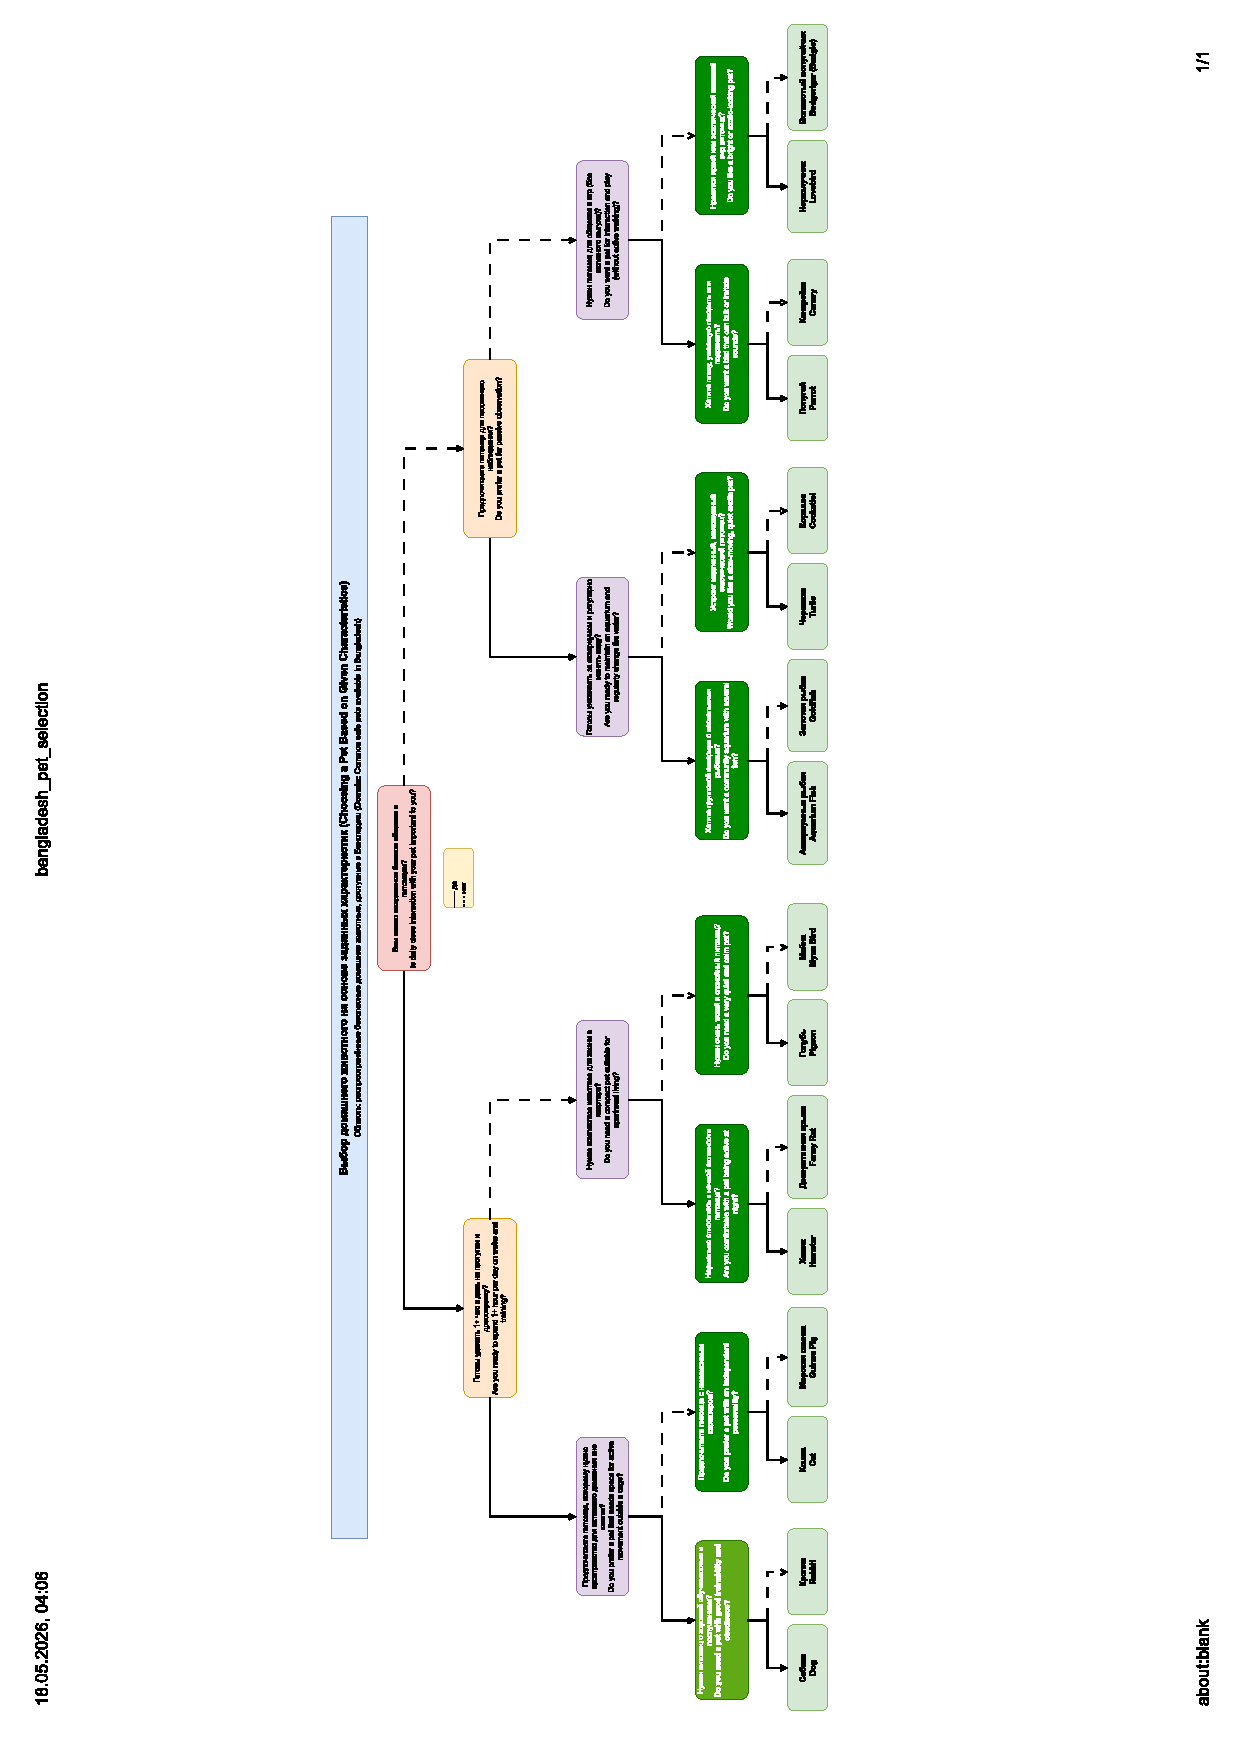
\includegraphics[width=\textwidth]{diagram.pdf}
	\caption{Бинарное дерево решений}
	\label{fig:diagram}
\end{figure}


\clearpage
\section{Особенности реализации}

Экспертная система реализована в среде CLIPS (C Language Integrated Production System) на основе продукционной модели. База знаний системы представлена набором из 31~правила (\texttt{defrule}): 15~правил реализуют узлы дерева решений и 16~правил~--- листовые узлы с рекомендациями. Рабочая память CLIPS хранит текущие факты о предпочтениях пользователя. Машина вывода автоматически выбирает и активирует подходящие правила. В данном разделе описаны ключевые функции и правила программы~\cite{telematika,habаров,gavrilova}.

\subsection{Общая функция задания вопроса и проверки ввода}

Функция \texttt{ask-question} является универсальной функцией запроса ввода у пользователя с проверкой корректности. Принимает текст вопроса \texttt{?question} и список допустимых значений \texttt{\$?allowed-values}. Выводит вопрос, считывает ответ функцией \texttt{read}, преобразует его к нижнему регистру функцией \texttt{lowcase}. Если ответ не входит в список допустимых значений (\texttt{member\$}), выводит сообщение об ошибке и повторяет запрос в цикле \texttt{while}. Возвращает принятый ответ. Код представлен в листинге~\ref{lst:askquestion}.

\begin{lstlisting}[language=CLIPS,
	caption={Функция ask-question},
	label=lst:askquestion]
(deffunction ask-question (?question $?allowed-values)
    (printout t ?question)
    (bind ?answer (read))
    (if (lexemep ?answer)
        then (bind ?answer (lowcase ?answer)))
    (while (not (member$ ?answer ?allowed-values)) do
        (printout t "  Invalid input. Please enter: " ?allowed-values crlf)
        (printout t ?question)
        (bind ?answer (read))
        (if (lexemep ?answer)
            then (bind ?answer (lowcase ?answer))))
    ?answer)
\end{lstlisting}

\subsection{Функция для вопросов типа да/нет}

Функция \texttt{yesno} является обёрткой над \texttt{ask-question}. Принимает только текст вопроса и вызывает \texttt{ask-question} с фиксированным списком допустимых значений (\texttt{yes no y n}). Нормализует ответ: если пользователь ввёл \texttt{y} или \texttt{yes}~--- возвращает символ \texttt{yes}, иначе~--- \texttt{no}. Это обеспечивает единообразие: все последующие правила системы работают только с символами \texttt{yes} и \texttt{no}, не зависимо от того, что именно ввёл пользователь. Код представлен в листинге~\ref{lst:yesno}.

\begin{lstlisting}[language=CLIPS,
	caption={Функция yesno},
	label=lst:yesno]
(deffunction yesno (?question)
    (bind ?response (ask-question ?question yes no y n))
    (if (or (eq ?response yes) (eq ?response y))
        then yes
        else no))
\end{lstlisting}

\subsection{Правило вывода рекомендации}

Правило \texttt{print-rec} имеет наивысший приоритет (\texttt{salience~1000}), что гарантирует его срабатывание раньше любого другого правила в момент появления в рабочей памяти факта \texttt{(rec~...)}. Правило выводит итоговую рекомендацию на экран, изымает факт \texttt{(rec~...)} из рабочей памяти и добавляет факт \texttt{(restart)}, запуская тем самым правило перезапуска. Код представлен в листинге~\ref{lst:printrec}.

\begin{lstlisting}[language=CLIPS,
	caption={Правило print-rec},
	label=lst:printrec]
(defrule print-rec
    (declare (salience 1000))
    ?rec <- (rec ?item)
    =>
    (printout t crlf "Recommended pet: " ?item crlf crlf)
    (retract ?rec)
    (assert (restart)))
\end{lstlisting}

\subsection{Правило перезапуска}

Правило \texttt{restart-system} срабатывает при появлении факта \texttt{(restart)} в рабочей памяти. Изымает факт \texttt{(restart)}, запрашивает у пользователя желание получить новую рекомендацию через функцию \texttt{ask-question} с валидацией ввода. При положительном ответе (\texttt{yes} или \texttt{y}) выводит заголовок программы и помещает в рабочую память факт с ответом на первый вопрос дерева, запуская новый сеанс. При отрицательном~--- выводит сообщение \texttt{Goodbye!} и останавливает машину вывода командой \texttt{halt}. Код представлен в листинге~\ref{lst:restart}.

\begin{lstlisting}[language=CLIPS,
	caption={Правило restart-system},
	label=lst:restart]
(defrule restart-system
    ?r <- (restart)
    =>
    (retract ?r)
    (bind ?a (ask-question "Would you like a new recommendation? (yes/no): "
                            yes no y n))
    (if (or (eq ?a yes) (eq ?a y))
        then
            (printout t crlf
                "=== Expert System: Pet Selection (Bangladesh) ===" crlf crlf)
            (assert (interaction
                (yesno "Is daily close interaction with your pet important to you? (yes/no): ")))
        else
            (printout t crlf "Goodbye!" crlf)
            (halt)))
\end{lstlisting}

\subsection{Правила дерева решений}

Каждый узел дерева реализован парой правил~--- для ответа «да» и для ответа «нет». Каждое правило: связывает совпавший факт переменной \texttt{?f}, изымает его из рабочей памяти (\texttt{retract}), задаёт следующий вопрос через \texttt{yesno} и добавляет новый факт (\texttt{assert}). Изъятие факта после срабатывания правила обеспечивает чистоту рабочей памяти: по завершении сеанса она полностью пуста, что гарантирует корректную работу при перезапуске. Стартовое правило \texttt{first} срабатывает только при полностью пустой рабочей памяти и выводит заголовок программы. В листинге~\ref{lst:rules} приведён фрагмент, демонстрирующий стартовое правило и правила первых двух уровней дерева; полная реализация представлена в Приложении~A1.

\begin{lstlisting}[language=CLIPS,
	caption={Фрагмент правил дерева решений (стартовое правило и первые два уровня)},
	label=lst:rules]
; Entry point — fires only when working memory is empty
(defrule first ""
    (not (interaction ?))
    (not (rec ?))
    (not (restart))
    =>
    (printout t "=== Expert System: Pet Selection (Bangladesh) ===" crlf crlf)
    (assert (interaction
        (yesno "Is daily close interaction with your pet important to you? (yes/no): "))))

; Level 2 — n2 (yes branch)
(defrule interaction-yes ""
    ?f <- (interaction yes) (not (rec ?)) =>
    (retract ?f)
    (assert (walks
        (yesno "Are you ready to spend 1+ hour per day on walks and training? (yes/no): "))))

; Level 2 — n3 (no branch)
(defrule interaction-no ""
    ?f <- (interaction no) (not (rec ?)) =>
    (retract ?f)
    (assert (passive
        (yesno "Do you prefer a pet for passive observation? (yes/no): "))))
\end{lstlisting}

\subsection{Правила-листья (рекомендации)}

16~правил-листьев реализуют листовые узлы дерева решений. Каждое правило проверяет наличие факта четвёртого уровня дерева и отсутствие факта \texttt{(rec~...)}. При срабатывании изымает свой факт и добавляет \texttt{(rec "Название животного")}. Это немедленно активирует правило \texttt{print-rec} с приоритетом 1000. Код представлен в листинге~\ref{lst:leaves}.

\begin{lstlisting}[language=CLIPS,
	caption={Правила-листья (фрагмент)},
	label=lst:leaves]
(defrule trainable-yes  "" ?f <- (trainable yes)  (not (rec ?)) =>
    (retract ?f) (assert (rec "Dog")))
(defrule trainable-no   "" ?f <- (trainable no)   (not (rec ?)) =>
    (retract ?f) (assert (rec "Rabbit")))

(defrule independent-yes "" ?f <- (independent yes) (not (rec ?)) =>
    (retract ?f) (assert (rec "Cat")))
(defrule independent-no  "" ?f <- (independent no)  (not (rec ?)) =>
    (retract ?f) (assert (rec "Guinea Pig")))

; ... (remaining 12 leaf rules follow the same pattern)

(defrule bright-yes "" ?f <- (bright yes) (not (rec ?)) =>
    (retract ?f) (assert (rec "Lovebird")))
(defrule bright-no  "" ?f <- (bright no)  (not (rec ?)) =>
    (retract ?f) (assert (rec "Budgerigar")))
\end{lstlisting}


\clearpage
\section{Результаты работы программы}

Результатом работы является готовая программа, реализованная в среде CLIPS. Запуск производится командами \texttt{(load "pet\_expert.clp")}, \texttt{(reset)}, \texttt{(run)} в интерпретаторе CLIPS. После запуска выводится заголовок и первый вопрос, находящийся в корне бинарного дерева. Пользователь отвечает \texttt{yes} (или \texttt{y}) для ответа «да» и \texttt{no} (или \texttt{n}) для ответа «нет». Программа проверяет корректность ввода: при неверном вводе выдаётся сообщение об ошибке и вопрос задаётся повторно. После прохождения четырёх уровней дерева система выводит рекомендацию и предлагает начать новый сеанс. Ниже представлены примеры работы программы.

На рис.~\ref{fig:run1} показан первый сеанс работы программы. Пользователь отвечает \texttt{y} на все четыре вопроса (путь да-да-да-да): система рекомендует \textit{Dog} (Собака). После рекомендации программа предлагает начать новый сеанс, демонстрируя также проверку корректности ввода при ответе на вопрос о перезапуске.

\begin{figure}[H]
	\centering
	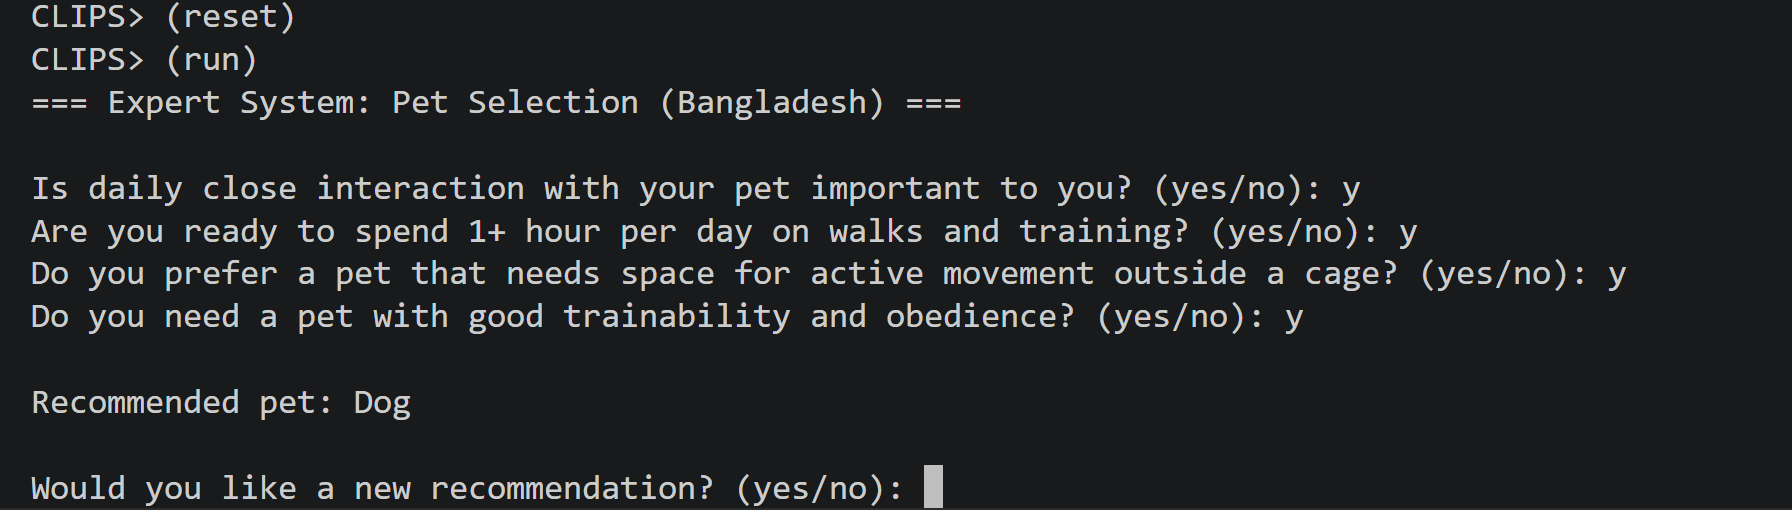
\includegraphics[width=\textwidth]{clips1.png}
	\caption{Пример №1: путь yes-yes-yes-yes, рекомендация --- Dog}
	\label{fig:run1}
\end{figure}

На рис.~\ref{fig:run2} представлен повторный сеанс с другими ответами. Программа демонстрирует корректную работу механизма перезапуска: рабочая память полностью очищается между сеансами, и система задаёт вопросы заново с первого уровня дерева.

\begin{figure}[H]
	\centering
	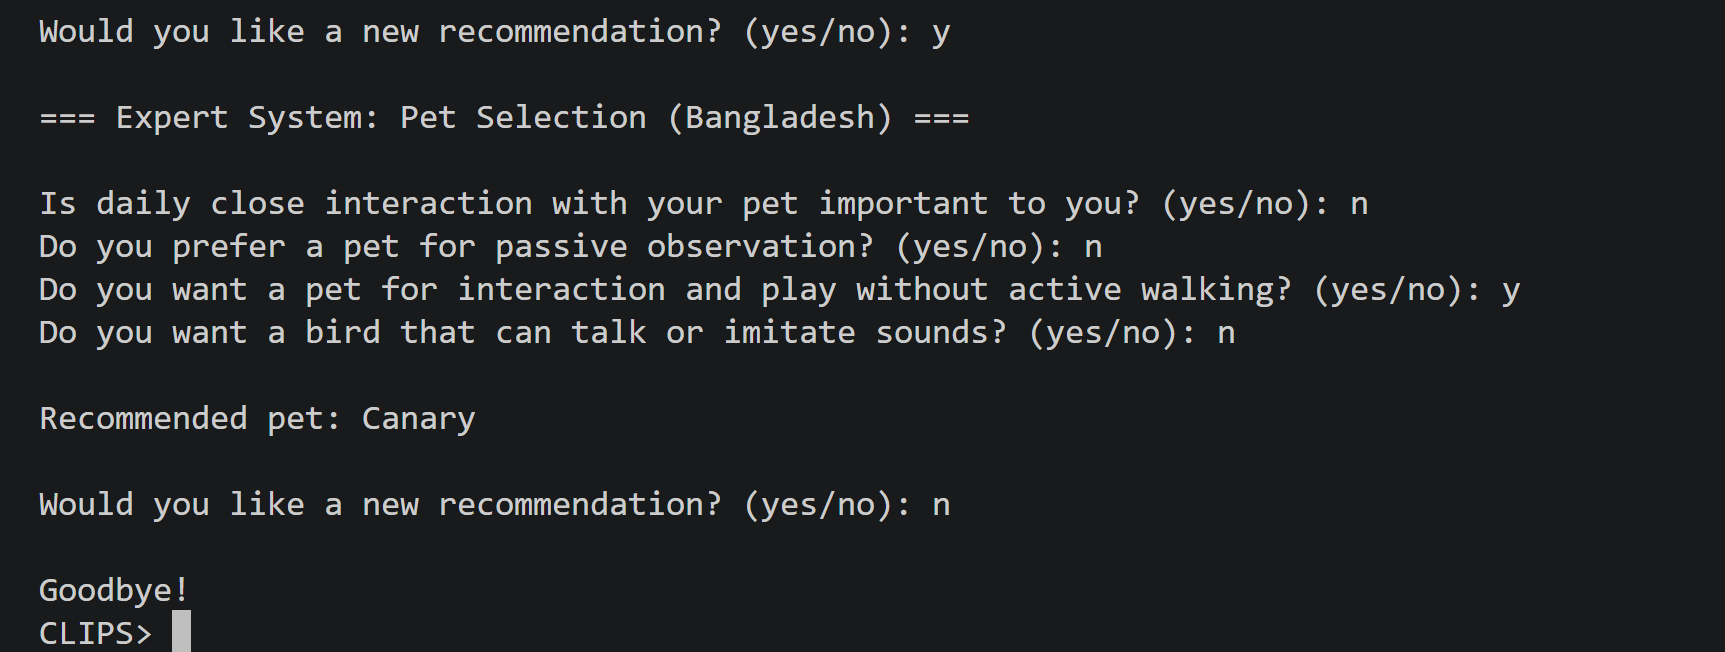
\includegraphics[width=\textwidth]{clips2.png}
	\caption{Пример №2: повторный сеанс с новыми ответами и завершение работы}
	\label{fig:run2}
\end{figure}


\clearpage
\section*{Заключение}

В результате курсовой работы была реализована экспертная система в среде CLIPS по теме «Выбор домашнего животного на основе заданных характеристик~(Бангладеш)»~\cite{dailystar,researchgate1,researchgate2}, представленная бинарным деревом решений со следующими числовыми характеристиками: количество узлов~--- 31, количество ярусов~--- 4, количество фактов~--- 16, количество правил~--- 15. Знания реализованной системы представлены в виде продукционной модели: база знаний состоит из 31~правила, рабочая память хранит текущие факты сеанса, машина вывода CLIPS автоматически управляет активацией правил. Данная система позволяет пользователю однозначно определить наиболее подходящего питомца, исходя из его образа жизни, жилищных условий и личных предпочтений.

\textbf{Достоинства}

Достоинства использования CLIPS и продукционной модели:
\begin{itemize}
	\item Знания (правила) отделены от механизма управления (машины вывода CLIPS): добавление нового узла в дерево требует только добавления новой пары правил, без изменения логики управления.
	\item Алгоритм обхода бинарного дерева эффективен: для получения рекомендации требуется ровно~4 вопроса в соответствии с числом ярусов дерева.
	\item Механизм приоритетов (\texttt{salience}) обеспечивает предсказуемый порядок срабатывания правил: правило вывода рекомендации всегда активируется первым.
\end{itemize}

\textbf{Недостатки}

\begin{itemize}
	\item При необходимости добавления или удаления узла необходимо перестроить дерево решений и добавить соответствующие правила, следовательно, система не является полностью гибкой.
	\item Экспертная система подходит для задач с ограниченным количеством факторов и простыми взаимодействиями; для более сложных алгоритмов требуются более продвинутые методы~--- семантические сети и фреймовые модели~\cite{gavrilova}.
\end{itemize}

\textbf{Масштабирование}

Программа может быть расширена путём добавления новых вопросов и животных, уточнения критериев классификации или расширения бинарного дерева решений. Другой способ масштабирования~--- переход к более сложным структурам представления знаний в CLIPS: использование \texttt{deftemplate} для структурированных фактов или подключение внешней базы знаний~\cite{habаров}.


\clearpage
\addcontentsline{toc}{section}{Список использованной литературы}
\begin{thebibliography}{99}

	\bibitem{dailystar}
	"Market for pet food, accessories growing"~/ The Daily Star.~---
	URL: \url{https://www.thedailystar.net/business/economy/news/market-pet-food-accessories-growing-3422306}
	(Дата обращения: 11.05.2026)

	\bibitem{researchgate1}
	The evolving paradigm of pet animal rearing in Bangladesh~/ ResearchGate.~---
	URL: \url{https://www.researchgate.net/publication/388758458}
	(Дата обращения: 11.05.2026)

	\bibitem{researchgate2}
	Navigating Pet Welfare in Bangladesh: A Multilayered Analysis of Ownership, Ethics and Service Accessibility~/ ResearchGate.~---
	URL: \url{https://www.researchgate.net/publication/398122556}
	(Дата обращения: 11.05.2026)

	\bibitem{bikroy}
	Animals \& Pets for sale in Bangladesh~/ Bikroy.com.~---
	URL: \url{https://bikroy.com/en/ads/bangladesh/pets-animals}
	(Дата обращения: 11.05.2026)

	\bibitem{bdfish}
	Aquarium Fishes of Bangladesh: Part-1~/ BdFISH Feature.~---
	URL: \url{https://en.bdfish.org/2011/01/aquarium-fish-bangladesh-1/}
	(Дата обращения: 11.05.2026)

	\bibitem{katabon}
	Katabon Online~--- Best Quality Pet Supplies (Dhaka pet market).~---
	URL: \url{https://katabononline.com/}
	(Дата обращения: 11.05.2026)

	\bibitem{dailybizeyе}
	The Rising Trend of Pet Ownership in Bangladesh~/ Daily Business Eye.~---
	URL: \url{https://www.dailybusinesseye.com/todayspaper/paper/4183}
	(Дата обращения: 11.05.2026)

	\bibitem{habаров}
	Хабаров~С.\,П. CLIPS~--- язык построения экспертных систем.~---
	Санкт-Петербург, 2013.~--- 80~с.

	\bibitem{gavrilova}
	Гаврилова~Т.\,А., Частиков~А.\,П. Разработка экспертных систем. Среда CLIPS.~---
	Санкт-Петербург: БХВ-Петербург, 2003.~--- 393~с.

	\bibitem{telematika}
	Секция «Телематика»~/ текст: электронный.~---
	URL: \url{https://tema.spbstu.ru/tgraph/}
	(Дата обращения: 11.05.2026)

\end{thebibliography}


\clearpage
\section*{Приложение A1. Файл pet\_expert.clp}
\addcontentsline{toc}{subsection}{Приложение A1. Файл pet\_expert.clp}
\label{app:clips}
\lstinputlisting[language=CLIPS, breaklines=true]{../pet_expert.clp}

\end{document}
